%
% A header that lets you compile a chapter by itself, or inside a larger document.
% Adapted from http://stackoverflow.com/questions/3655454/conditional-import-in-latex
%
%
%Use \inbpdocument and \outbpdocument in your individual files, in place of \begin{document} and \end{document}. In your main file, put in a \def \ismaindoc {} before including or importing anything.
%
% David Duvenaud
% June 2011
% 
% ======================================
%
%


\ifx\ismaindoc\undefined
	\newcommand{\inbpdocument}{
		\def \ismaindoc {}
		% Use this header if we are compiling by ourselves.
		\documentclass[a4paper,11pt,authoryear,index]{common/PhDThesisPSnPDF}
		
%\usepackage{draftwatermark}
%\SetWatermarkLightness{0.95}

% ******************************************************************************
% ****************************** Custom Margin *********************************

% Add `custommargin' in the document class options to use this section
% Set {innerside margin / outerside margin / topmargin / bottom margin}  and
% other page dimensions

\ifsetMargin
\else
    \RequirePackage[left=37mm,right=30mm,top=35mm,bottom=30mm]{geometry}
    \setFancyHdr % To apply fancy header after geometry package is loaded
\fi


%\chead{Unfinished draft}
%\cfoot{\texttt{Unfinished draft - compiled on \today{} at \currenttime}}

% *****************************************************************************
% ******************* Fonts (like different typewriter fonts etc.)*************

% Add `customfont' in the document class option to use this section

\ifsetFont
\else
    % Set your custom font here and use `customfont' in options. Leave empty to
    % load computer modern font (default LaTeX font).  

    \RequirePackage{libertine} 
\fi

% *****************************************************************************
% *************************** Bibliography  and References ********************

%\usepackage{cleveref} %Referencing without need to explicitly state fig /table

% Add `custombib' in the document class option to use this section
\ifsetBib % True, Bibliography option is chosen in class options
\else % If custom bibliography style chosen then load bibstyle here

   \RequirePackage[square, sort, numbers, authoryear]{natbib} % CustomBib

% If you would like to use biblatex for your reference management, as opposed to the default `natbibpackage` pass the option `custombib` in the document class. Comment out the previous line to make sure you don't load the natbib package. Uncomment the following lines and specify the location of references.bib file

% \RequirePackage[backend=biber, style=numeric-comp, citestyle=numeric, sorting=nty, natbib=true]{biblatex}
% \bibliography{References/references} %Location of references.bib only for biblatex

\fi


% changes the default name `Bibliography` -> `References'
\renewcommand{\bibname}{References}


% *****************************************************************************
% *************** Changing the Visual Style of Chapter Headings ***************
% Uncomment the section below. Requires titlesec package.

%\RequirePackage{titlesec}
%\newcommand{\PreContentTitleFormat}{\titleformat{\chapter}[display]{\scshape\Large}
%{\Large\filleft{\chaptertitlename} \Huge\thechapter}
%{1ex}{}
%[\vspace{1ex}\titlerule]}
%\newcommand{\ContentTitleFormat}{\titleformat{\chapter}[display]{\scshape\huge}
%{\Large\filleft{\chaptertitlename} \Huge\thechapter}{1ex}
%{\titlerule\vspace{1ex}\filright}
%[\vspace{1ex}\titlerule]}
%\newcommand{\PostContentTitleFormat}{\PreContentTitleFormat}
%\PreContentTitleFormat


% *****************************************************************************
% **************************** Custom Packages ********************************
% *****************************************************************************


% ************************* Algorithms and Pseudocode **************************

%\usepackage{algpseudocode} 


% ********************Captions and Hyperreferencing / URL **********************

% Captions: This makes captions of figures use a boldfaced small font. 
%\RequirePackage[small,bf]{caption}

\RequirePackage[labelsep=space,tableposition=top]{caption} 
%\renewcommand{\figurename}{Figure} %to support older versions of captions.sty
\captionsetup{belowskip=12pt,aboveskip=4pt}

% ************************ Formatting / Footnote *******************************

%\usepackage[perpage]{footmisc} %Range of footnote options 


% ****************************** Line Numbers **********************************

%\RequirePackage{lineno}
%\linenumbers

% ************************** Graphics and figures *****************************

%\usepackage{rotating}
%\usepackage{wrapfig}
%\usepackage{float}
\usepackage{subfig} %note: subfig must be included after the `caption` package. 


% ********************************* Table **************************************

%\usepackage{longtable}
%\usepackage{multicol}
%\usepackage{multirow}
%\usepackage{tabularx}


% ***************************** Math and SI Units ******************************

\usepackage{amsfonts}
\usepackage{amsmath}
\usepackage{amssymb}
%\usepackage{siunitx} % use this package module for SI units


% ******************************************************************************
% ************************* User Defined Commands ******************************
% ******************************************************************************

% *********** To change the name of Table of Contents / LOF and LOT ************

%\renewcommand{\contentsname}{My Table of Contents}
%\renewcommand{\listfigurename}{List of figures}
%\renewcommand{\listtablename}{List of tables}


% ********************** TOC depth and numbering depth *************************

\setcounter{secnumdepth}{2}
\setcounter{tocdepth}{2}

% ******************************* Nomenclature *********************************

% To change the name of the Nomenclature section, uncomment the following line

%\renewcommand{\nomname}{Symbols}


% ********************************* Appendix ***********************************

% The default value of both \appendixtocname and \appendixpagename is `Appendices'. These names can all be changed via: 

%\renewcommand{\appendixtocname}{List of appendices}
%\renewcommand{\appendixname}{Appndx}

		% All my custom preamble stuff.  Shouldn't overlap with anything in official-preamble


% Paths to figure and table directories.
\newcommand{\symmetryfigsdir}{figures/symmetries}
\newcommand{\topologyfiguresdir}{figures/topology}
\newcommand{\infinitefiguresdir}{figures/infinite}
\newcommand{\grammarfiguresdir}{figures/grammar}
\newcommand{\introfigsdir}{figures/intro}
\newcommand{\gplvmfiguresdir}{figures/gplvm}
\newcommand{\warpedfiguresdir}{figures/warped-mixtures}
\newcommand{\deeplimitsfiguresdir}{figures/deep-limits}
\newcommand{\quadraturefigsdir}{figures/quadrature}
\newcommand{\additivefigsdir}{figures/additive}
\newcommand{\decompfigsdir}{figures/decomp}
\newcommand{\examplefigsdir}{figures/worked-example}


\usepackage{bm}  % for warped mixtures - is this necessary?
\usepackage{booktabs}
\usepackage{tabularx}
\usepackage{multirow}
\usepackage{datetime}
\renewcommand{\tabularxcolumn}[1]{>{\arraybackslash}m{#1}}
\usepackage{relsize}
\usepackage{graphicx}
\usepackage{amsmath,amssymb,textcomp}
\usepackage{nicefrac}
\usepackage{amsthm}
\usepackage{tikz}
\usetikzlibrary{arrows}
\usetikzlibrary{calc}
\usepackage{nth}
\usepackage{rotating}
\usepackage{array}
\usepackage{fp}
\usepackage[hyperpageref]{backref}
\def\foo{\hspace{\fill}\mbox{}\linebreak[0]\hspace*{\fill}}
\renewcommand*{\backref}[1]{}
\renewcommand*{\backrefalt}[4]{%
\ifcase #1 %
%
\or
\foo(page #2)%
\else
\foo(pages #2)%
\fi
}

\usepackage{cleveref}
\crefname{equation}{equation}{equations}


%% For submission, make all render blank.
%%%%%%%%%%%%%%%%%%%%%%%%%%%%%%%%%%%%%%%%%%%%%%%%%%%%%%%%%%
%%%% EDITING HELPER FUNCTIONS  %%%%%%%%%%%%%%%%%%%%%%%%%%%
%%%%%%%%%%%%%%%%%%%%%%%%%%%%%%%%%%%%%%%%%%%%%%%%%%%%%%%%%%

%% NA: needs attention (rough writing whose correctness needs to be verified)
%% TBD: instructions for how to fix a gap ("Describe the propagation by ...")
%% PROBLEM: bug or missing crucial bit 

%% use \fXXX versions of these macros to put additional explanation into a footnote.  
%% The idea is that we don't want to interrupt the flow of the paper or make it 
%% impossible to read because there are a bunch of comments.

%% NA's (and TBDs, those less crucially) should be written so 
%% that they flow with the text.

\definecolor{WowColor}{rgb}{.75,0,.75}
\definecolor{SubtleColor}{rgb}{0,0,.50}

% inline
\newcommand{\NA}[1]{\textcolor{SubtleColor}{ {\tiny \bf ($\star$)} #1}}
\newcommand{\LATER}[1]{\textcolor{SubtleColor}{ {\tiny \bf ($\dagger$)} #1}}
\newcommand{\TBD}[1]{\textcolor{SubtleColor}{ {\tiny \bf (!)} #1}}
\newcommand{\PROBLEM}[1]{\textcolor{WowColor}{ {\bf (!!)} {\bf #1}}}

% as margin notes

\newcounter{margincounter}
\newcommand{\displaycounter}{{\arabic{margincounter}}}
\newcommand{\incdisplaycounter}{{\stepcounter{margincounter}\arabic{margincounter}}}

\newcommand{\fTBD}[1]{\textcolor{SubtleColor}{$\,^{(\incdisplaycounter)}$}\marginpar{\tiny\textcolor{SubtleColor}{ {\tiny $(\displaycounter)$} #1}}}

\newcommand{\fPROBLEM}[1]{\textcolor{WowColor}{$\,^{((\incdisplaycounter))}$}\marginpar{\tiny\textcolor{WowColor}{ {\bf $\mathbf{((\displaycounter))}$} {\bf #1}}}}

\newcommand{\fLATER}[1]{\textcolor{SubtleColor}{$\,^{(\incdisplaycounter\dagger)}$}\marginpar{\tiny\textcolor{SubtleColor}{ {\tiny $(\displaycounter\dagger)$} #1}}}

%\renewcommand{\LATER}[1]{}
%\renewcommand{\fLATER}[1]{}
%\renewcommand{\TBD}[1]{}
%\renewcommand{\fTBD}[1]{}
%\renewcommand{\PROBLEM}[1]{}
%\renewcommand{\fPROBLEM}[1]{}
%\renewcommand{\NA}[1]{}


% HUMBLE WORDS: shown slightly smaller when in normal text
% Thanks to Christian Steinruecken!

% HUMBLE WORDS: shown slightly smaller when in normal text
%
\makeatletter%
%\def\@humbleformat#1{{\fontsize{}{1em}\selectfont #1}}
%\def\@humbleformat#1{\textsmaller{#1}}%
\newlength{\nonHumbleHeight}
\def\@humbleformat#1{{\settoheight{\nonHumbleHeight}{#1}\resizebox{!}{0.94\nonHumbleHeight}{#1}}}%
\def\@idxhumbleformat#1{{\relscale{0.95}{#1}}}%
%\def\@humbleformat#1{{#1}}%
\def\declareHumble#1#2{%
  \expandafter\def\csname #1\endcsname{\@humbleformat{#2}}%
  \expandafter\def\csname s#1\endcsname{{#2}}%
  \expandafter\def\csname idx#1\endcsname{{\@idxhumbleformat{#2}}}%
}%
\def\humble#1{\@humbleformat{#1}}%
\def\idxhumble#1{\@idxhumbleformat{#1}}%
\makeatother%

% Convenient indexing for humble abbreviations
\def\humbleindex#1#2{\index{#1@\idxhumble{#1}}}



% TODO: Clean up duplicates
\declareHumble{ANOVA}{ANOVA}
\declareHumble{ARD}{ARD}
\declareHumble{BIC}{BIC}
\declareHumble{BMC}{BMC}
\declareHumble{bq}{BQ}
\declareHumble{CRP}{CRP}
\declareHumble{dirpro}{DP}
\declareHumble{HDMR}{HDMR}
\declareHumble{GAM}{GAM}
\declareHumble{GEM}{GEM}
\declareHumble{GMM}{GMM}
\declareHumble{gplvm}{GP-LVM}
\declareHumble{gpml}{GPML}
\declareHumble{GPML}{GPML}
\declareHumble{gprn}{GPRN}
\declareHumble{gpt}{GP}
\declareHumble{gp}{GP}
\declareHumble{HKL}{HKL}
\declareHumble{HMC}{HMC}
\declareHumble{ibp}{IBP}
\declareHumble{iGMM}{iGMM}
\declareHumble{iwmm}{iWMM}
\declareHumble{kCP}{CP}
\declareHumble{kCW}{CW}
\declareHumble{kC}{C}
\declareHumble{KDE}{KDE}
\declareHumble{kLin}{Lin}
\declareHumble{KPCA}{KPCA}
\declareHumble{kPer}{Per}
\declareHumble{kRQ}{RQ}
\declareHumble{kSE}{SE}
\declareHumble{kWN}{WN}
\declareHumble{Lin}{Lin}
\declareHumble{LBFGS}{L-BFGS}
\declareHumble{mcmc}{MCMC}
\declareHumble{MKL}{MKL}
\declareHumble{MLP}{MLP}
\declareHumble{MSE}{MSE}
\declareHumble{Per}{Per}
\declareHumble{RMSE}{RMSE}
\declareHumble{RQ}{RQ}
\declareHumble{SBQ}{SBQ}
\declareHumble{seard}{SE-ARD}
\declareHumble{sefull}{SE-\textnormal{full}}
\declareHumble{SEGP}{SE-GP}
\declareHumble{SE}{SE}
\declareHumble{SNR}{SNR}
\declareHumble{SSANOVA}{SS-ANOVA}
\declareHumble{SVM}{SVM}

\newcommand{\kSig}{\boldsymbol\sigma}

\def\subexpr{{\cal S}}
\def\baseker{{\cal B}}
\def\numWinners{k}

\def\ie{i.e.\ }
\def\eg{e.g.\ }
\def\etc{etc.\ }
\let\oldemptyset\emptyset
\let\emptyset 0




% Unify notation between neural-net land and GP-land.
\newcommand{\hphi}{h}
\newcommand{\hPhi}{\vh}
\newcommand{\walpha}{w}
\newcommand{\wboldalpha}{\bw}
\newcommand{\wcapalpha}{\vW}
\newcommand{\lengthscale}{w}

\newcommand{\layerindex}{\ell}



\newcommand{\gpdrawbox}[1]{
\setlength\fboxsep{0pt}
\hspace{-0.15in} 
\fbox{
\includegraphics[width=0.464\columnwidth]{\deeplimitsfiguresdir/deep_draws/deep_gp_sample_layer_#1}
}}



\newcommand{\procedurename}{ABCD}
\newcommand{\genText}[1]{{\sf #1}}



\newcommand{\asdf}{$^{\textnormal{th}}$}

\newcommand{\binarysum}{\sum_{\bf{x} \in \{0,1\}^D}}
\newcommand{\expect}{\mathbb{E}}
\newcommand{\expectargs}[2]{\mathbb{E}_{#1} \left[ {#2} \right]}
\newcommand{\var}{\mathbb{V}}
\newcommand{\varianceargs}[2]{\mathbb{V}_{#1} \left[ {#2} \right]}
\newcommand{\cov}{\operatorname{cov}}
\newcommand{\Cov}{\operatorname{Cov}}
\newcommand{\covargs}[2]{\cov \left[ {#1}, {#2} \right]}
\newcommand{\variance}{\mathbb{V}}
\newcommand{\vecop}[1]{\operatorname{vec} \left( {#1} \right)}

\newcommand{\covarianceargs}[2]{\Cov_{#1} \left[ {#2} \right]}
\newcommand{\colvec}[2]{\left[ \begin{array}{c} {#1} \\ {#2} \end{array} \right]}
\newcommand{\tbtmat}[4]{\left[ \begin{array}{cc} {#1} & {#2} \\ {#3} & {#4} \end{array} \right]}

%\newcommand{\covskinny}[2]{\var\!\left(#1\middle\vert#2\right)} 

\newcommand{\acro}[1]{{\humble{#1}}}
%\newcommand{\vect}[1]{\boldsymbol{#1}}
\newcommand{\vect}[1]{{\bf{#1}}}
\newcommand{\mat}[1]{\mathbf{#1}}
\newcommand{\pderiv}[2]{\frac{\partial #1}{\partial #2}}
\newcommand{\npderiv}[2]{\nicefrac{\partial #1}{\partial #2}}

\newcommand{\pha}{^{\phantom{:}}}

\newcommand{\argmin}{\operatornamewithlimits{argmin}}
\newcommand{\argmax}{\operatornamewithlimits{argmax}}

% The following designed for probabilities with long arguments

\newcommand{\Prob}[2]{P\!\left(\,#1\;\middle\vert\;#2\,\right)}
\newcommand{\ProbF}[3]{P\!\left(\,#1\!=\!#2\;\middle\vert\;#3\,\right)}
\newcommand{\p}[2]{p\!\left(#1\middle\vert#2\right)}
\newcommand{\po}[1]{p\!\left(#1\right)}
\newcommand{\pF}[3]{p\!\left(\,#1\!=\!#2\;\middle\vert\;#3\,\right)} 
\newcommand{\mean}[2]{{m}\!\left(#1\middle\vert#2\right)}



\newcommand{\valpha}{\boldsymbol{\alpha}}
\newcommand{\va}{\vect{a}}
\newcommand{\vA}{\vect{A}}
\newcommand{\vB}{\mat{B}}
\newcommand{\vb}{\vect{b}}
\newcommand{\vC}{\mat{C}}
\newcommand{\vc}{\vect{c}}
\newcommand{\vecf}{\boldsymbol{f}}
\newcommand{\vell}{\vect{\ell}}
\newcommand{\vepsilon}{\boldsymbol{\epsilon}}
\newcommand{\veps}{\boldsymbol{\epsilon}}
\newcommand{\ve}{\boldsymbol{\epsilon}}
\newcommand{\vf}{\vecf}
\newcommand{\vg}{\vect{g}}
\newcommand{\vh}{\vect{h}}
\newcommand{\vI}{\mat{I}}
\newcommand{\vK}{\mat{K}}
\newcommand{\vk}{\vect{k}}
\newcommand{\vL}{\mat{L}}
\newcommand{\vl}{\vect{l}}
\newcommand{\vmu}{\boldsymbol{\mu}}
\newcommand{\vone}{\vect{1}}
\newcommand{\vphi}{\boldsymbol{\phi}}
\newcommand{\vpi}{\boldsymbol{\pi}}
\newcommand{\vq}{\vect{q}}
\newcommand{\vR}{\mat{R}}
\newcommand{\vr}{\vect{r}}
\newcommand{\vsigma}{\boldsymbol{\sigma}}
\newcommand{\vSigma}{\mat{\Sigma}}
\newcommand{\vS}{\mat{S}}
\newcommand{\vs}{\vect{s}}
\newcommand{\vtheta}{\boldsymbol{\theta}}
\newcommand{\vu}{\vect{u}}
\newcommand{\vV}{\mat{V}}
\newcommand{\vW}{\mat{W}}
\newcommand{\vw}{\vect{w}}
\newcommand{\vX}{\mat{X}}
\newcommand{\vx}{\vect{x}}
\newcommand{\vY}{\mat{Y}}
\newcommand{\vy}{\vect{y}}
\newcommand{\vzero}{\vect{0}}
\newcommand{\vZ}{\mat{Z}}
\newcommand{\vz}{\vect{z}}


\newcommand{\netweights}{\alpha}
\newcommand{\vnetweights}{\valpha}

\newcommand{\He}{\mathcal{H}}
\newcommand{\normx}[2]{\left\|#1\right\|_{#2}}
\newcommand{\Hnorm}[1]{\normx{#1}{\He}}
\newcommand{\mmd}{{\rm MMD}}


\newcommand{\mf}{\bar{\vf}}

%\newcommand{\mf}{\mu} %{\bar{\ell}}
\newcommand{\lf}{f} % Likelihood function
\newcommand{\st}{_\star}

% from simpler log-bq writeup
\newcommand{\lftwo}{{\log \ell}}
\newcommand{\mftwo}{{\bar \ell}}
\newcommand{\loggp}{{\log\acro{GP}}}%| \bX, \vy )}}
\newcommand{\loggpdist}{{\acro{GP}(\lftwo)}}%| \vX, \vy )}}


\newcommand{\inv}{^{{\mathsmaller{-1}}}}
\newcommand{\tohalf}{^{{\mathsmaller{\nicefrac{1}{2}}}}}

\newcommand{\Normal}{\mathcal{N}}
\newcommand{\N}[3]{\mathcal{N}\!\left(#1 \middle| #2,#3\right)}
\newcommand{\Nt}[2]{\mathcal{N}\!\left(#1,#2\right)}
\newcommand{\NT}[2]{\mathcal{N}\!\left(#1,#2\right)}
\newcommand{\GPdist}[3]{\mathcal{GP}\!\left(#1 \, \middle| \, #2, #3 \right)}
\newcommand{\bN}[3]{\mathcal{N}\big(#1 \middle| #2,#3\big)}
\newcommand{\boldN}[3]{\text{\textbf{\mathcal{N}}}\big(#1;#2,#3\big)}
\newcommand{\ones}[1]{\mat{1}_{#1}}
\newcommand{\eye}[1]{\mat{E}_{#1}}
\newcommand{\tra}{^{\mathsf{T}}}
%\newcommand{\tra}{^{\top}}
%\mathsf{T}
\newcommand{\trace}{\operatorname{tr}}
\newcommand{\shift}{\operatorname{shift}}
\renewcommand{\mod}{\operatorname{mod}}
\newcommand{\deq}{:=}
\newcommand{\oneofk}{\operatorname{one-of-k}}
%\newcommand{\degree}{^\circ}

\newcommand{\GPt}[2]{\mathcal{GP}\!\left(#1,#2\right)}
%\newcommand{\GPt}[2]{\gp\!\left(#1,#2\right)}

\DeclareMathOperator{\tr}{tr}
\DeclareMathOperator{\chol}{chol}
\DeclareMathOperator{\diag}{diag}

\newenvironment{narrow}[2]{%
  \begin{list}{}{%
  \setlength{\topsep}{0pt}%
  \setlength{\leftmargin}{#1}%
  \setlength{\rightmargin}{#2}%
  \setlength{\listparindent}{\parindent}%
  \setlength{\itemindent}{\parindent}%
  \setlength{\parsep}{\parskip}}%
\item[]}{\end{list}}



\newcommand{\dist}{\ \sim\ }
\def\given{\,|\,}

% Table stuff
\newcolumntype{C}[1]{>{\centering\let\newline\\\arraybackslash\hspace{0pt}}m{#1}}
\newcolumntype{L}[1]{>{\raggedright\let\newline\\\arraybackslash\hspace{0pt}}m{#1}}
\newcolumntype{R}[1]{>{\raggedleft\let\newline\\\arraybackslash\hspace{0pt}}m{#1}}


\def\ie{i.e.\ }
\def\eg{e.g.\ }
\def\iid{i.i.d.\ }
%\def\simiid{\sim_{\mbox{\tiny iid}}}
\def\simiid{\overset{\mbox{\tiny iid}}{\sim}}
\def\simind{\overset{\mbox{\tiny \textnormal{ind}}}{\sim}}
\def\eqdist{\stackrel{\mbox{\tiny d}}{=}}
%\newcommand{\distas}[1]{\mathbin{\overset{#1}{\kern \z@ \sim}}}
%TODO: fix this - it worked outside the thesis!
\newcommand{\distas}[1]{\mathbin{\overset{#1}{\sim}}}

\def\Reals{\mathbb{R}}

\def\Uniform{\mbox{\rm Uniform}}
\def\Bernoulli{\mbox{\rm Bernoulli}}
\def\GP{\mathcal{GP}}
\def\GPLVM{\mathcal{GP-LVM}}




% Kernel stuff

\def\iva{\vect{\inputVar}}
\def\ivaone{\inputVar}
\def\inputVar{x}
\def\InputVar{X}
\def\InputSpace{\mathcal{X}}
\def\outputVar{y}
\def\OutputSpace{\mathcal{Y}}
\def\function{f}
\def\kernel{k}
\def\KernelMatrix{K}
\def\SumKernel{\sum}
\def\ProductKernel{\prod}
\def\expression{e}
\def\feat{\vh}

\newcommand{\kerntimes}{ \! \times \!}
\newcommand{\kernplus}{ \, + \,}


% Proof stuff
\theoremstyle{plain}
\newtheorem{theorem}{Theorem}[section]
\newtheorem{lemma}[theorem]{Lemma}
\newtheorem{prop}[theorem]{Proposition}
\newtheorem{proposition}{Proposition}
\newtheorem*{cor}{Corollary}

% For infinite bq
\newcommand{\iv}{\theta}
\newcommand{\viv}{\vtheta}

% For intro chapter
\newcommand{\funcval}{\vf(\vX)}
\newcommand{\testpoint}{{\vx^\star}}

\newcommand{\underwrite}[2]{{\underbrace{#1}_{\textnormal{#2}}}}



% For kernel figures
\newcommand{\fhbig}{2cm}%
\newcommand{\fwbig}{3cm}%
\newcommand{\kernpic}[1]{\includegraphics[height=\fhbig,width=\fwbig]{\grammarfiguresdir/structure_examples/#1}}%
\newcommand{\kernpicr}[1]{\rotatebox{90}{\includegraphics[height=\fwbig,width=\fhbig]{\grammarfiguresdir/structure_examples/#1}}}%
\newcommand{\addkernpic}[1]{{\includegraphics[height=\fhbig,width=\fwbig]{\grammarfiguresdir/additive_multi_d/#1}}}%
\newcommand{\largeplus}{\tabbox{{\Large+}}}%
\newcommand{\largeeq}{\tabbox{{\Large=}}}%
\newcommand{\largetimes}{\tabbox{{\Large$\times$}}}%
\newcommand{\fixedx}{$x$ (with $x' = 1$)}%


		% ************************ Thesis Information & Meta-data **********************

%% The title of the thesis
%\title{Structured Gaussian Process Models} 
%\title{Automatic Model Construction \\ through \\ Structured Gaussian Processes}
%\title{Automatic Model-Building \\ through \\ Structured Gaussian Processes}
%\title{Automatic Modeling \\ with \\ Structured Gaussian Processes}    
\title{Automatic Model Construction \\ with Gaussian Processes}
%\title{Automatic Model Construction}
%\title{Automating Statistical Model Construction}


%\texorpdfstring is used for PDF metadata. Usage:
%\texorpdfstring{LaTeX_Version}{PDF Version (non-latex)} eg.,
%\texorpdfstring{$sigma$}{sigma}

%% The full name of the author
\author{David Kristjanson Duvenaud}

%% Department (eg. Department of Engineering, Maths, Physics)
%\dept{Department of Engineering}

%% University and Crest
\university{University of Cambridge}
\crest{
\includegraphics[width=0.25\textwidth]{University_Crest}}

%% You can redefine the submission text:
% Default as per the University guidelines: This dissertation is submitted for
% the degree of Doctor of Philosophy
%\renewcommand{\submissiontext}{change the default text here if needed}

%% Full title of the Degree 
\degree{Doctor of Philosophy}
 
%% College affiliation (optional)
\college{Pembroke College}

%% Submission date
\degreedate{June 2014} 

%% Meta information
\subject{LaTeX} \keywords{{LaTeX} {PhD Thesis} {Engineering} {University of Cambridge}}



		\begin{document}
	}	
	\newcommand{\outbpdocument}[1]{

		% Fake chapters so references aren't broken
\label{ch:intro}                
\label{ch:kernels}
\label{ch:grammar}
\label{ch:description}
\label{ch:additive}
\label{ch:deeplimits}
\label{ch:discussion}
		%\bibliographystyle{common/CUEDthesis}
		\bibliographystyle{plainnat}
		\bibliography{references.bib}
		\end{document}
	}	
\else
	%If we're inside another document, no need to re-start the document.
	\ifx\inbpdocument\undefined
		\newcommand{\inbpdocument}{}
		\newcommand{\outbpdocument}[1]{}
	\fi
\fi

\inbpdocument


\chapter{Automatic Model Construction}
\label{ch:grammar}

\begin{quotation}
``It would be very nice to have a formal apparatus that gives us some `optimal' way of recognizing unusual phenomena and inventing new classes of hypotheses that are most likely to contain the true one; but this remains an art for the creative human mind.''

\defcitealias{Jaynes85highlyinformative}{ -- E. T.  Jaynes (1985)}
\hspace*{\fill}\citetalias{Jaynes85highlyinformative}
\end{quotation}


In \cref{ch:kernels}, we saw that the choice of kernel determines the type of structure that can be learned by a \gp{} model, and that a wide variety of models could be constructed by adding and multiplying a few base kernels together.
However, we did not answer the difficult question of which kernel to use for a given problem.
Even for experts, choosing the kernel in \gp{} regression remains something of a black art.

The contribution of this chapter is to show a way to automate the process of building kernels for \gp{} models.
We do this by defining an open-ended space of kernels built by adding and multiplying together kernels from a fixed set.
We then define a procedure to search over this space to find a kernel which matches the structure in the data.

Searching over such a large, structured model class has two main benefits.
First, this procedure has good predictive accuracy, since it tries out a large number of different regression models.
Second, this procedure can sometimes discover interpretable structure in datasets.
Because \gp{} posteriors can be decomposed (as in \cref{sec:concrete}), the resulting structures can be examined visually.
In \cref{ch:description}, we also show how to automatically generate English-language descriptions of the resulting models.

%\paragraph{Attribution}

This chapter is based on work done in collaboration with James Robert Lloyd, Roger Grosse, Joshua B. Tenenbaum, and Zoubin Ghahramani.
It was published in \citet{DuvLloGroetal13} and \citet{LloDuvGroetal14}.
Myself, James Lloyd and Roger Grosse jointly developed the idea of searching through a grammar-based language of \gp{} models, inspired by \citet{grosse2012exploiting}, 
and wrote the first versions of the code together.
James Lloyd ran most of the experiments, and I constructed most of the figures.
%I produced all of the figures.
%Zoubin Ghahramani and Josh Tenenbaum provided many conceptual insights, as well as suggestions about how the resulting procedure could be most fruitfully applied.

%\paragraph{Automatic statistician:} The work appearing in chapter \ref{ch:description} was written in collaboration with James Robert Lloyd, Roger Grosse, Joshua B. Tenenbaum, Zoubin Ghahramani, and was published in .
%The procedure translating kernels into adjectives grew out of discussions between James and myself.
%James Lloyd wrote the code to automatically generate reports, and ran all of the experiments.
%The text was written mainly by myself, James Lloyd, and Zoubin Ghahramani, with many helpful contributions and suggestions from Roger Grosse and Josh Tenenbaum.


%Section \ref{sec:Structure} outlines some commonly used kernel families as well as ways in which they can be composed. 
%Our grammar over kernels and our proposed structure discovery algorithm are described in Section \ref{sec:Search}. 
%Section \ref{sec:related_work} situates our work in the context of other nonparametric regression, kernel learning, and structure discovery methods.
%We evaluate our methods on synthetic datasets, time series analysis, and high-dimensional prediction problems in Sections \ref{sec:synthetic} through \ref{sec:quantitative}, respectively.




\section{Ingredients of an automatic statistician}
\label{sec:ingredients}
\citet{gelman2013philblogpost} asks: ``How can an artificial intelligence do statistics? \dots It needs not just an inference engine, but also a way to construct new models and a way to check models. Currently, those steps are performed by humans, but the AI would have to do it itself''.
%
This section will discuss the different parts we think are required to build an artificial intelligence that can do statistics.

\begin{enumerate}
\item {\bf An open-ended language of models.}
Many learning algorithms consider all models in a class of fixed size.
For example, graphical model learning algorithms \citep{Friedman03,Eaton07_uai} search over different connectivity graphs for a given set of nodes.
Such methods can be powerful, but human statisticians are sometimes capable of deriving \emph{novel} model classes when required.
An automatic search through an open-ended class of models can achieve some of this flexibility, %growing the complexity of the model as needed, 
possibly combining existing structures in novel ways.

\item {\bf A search through model space.}
%An open-ended space of models cannot be searched exhaustively.
Any procedure which eventually considers any model in an open-ended space must start with relatively simple models before moving on to more complex ones.
%Any model search procedure which visits every model eventually cannot start by guessing the 
Thus any search strategy capable of building arbitrarily complex models is likely to resemble an iterative model-building procedure.
Just as human researchers iteratively refine their models, search procedures can propose new candidate models based on the results of previous model fits.

\item {\bf A model comparison procedure.}
Search strategies requires an objective to optimize.
In this work, we use approximate marginal likelihood to compare models, penalizing complexity using the Bayesian Information Criterion as a heuristic.
More generally, an automatic statistician needs to somehow check the models it has constructed.
%, and formal procedures from model checking provide a way for it to do this.
\citet{gelman2012philosophy} review the literature on model checking.

\item {\bf A model description procedure.}
Part of the value of statistical models comes from helping humans to understand a dataset or a phenomenon.
Furthermore, a clear description of the statistical structure found in a dataset helps a user to notice when the dataset has errors, the wrong question was asked, the model-building procedure failed to capture known structure, a relevant piece of data or constraint is missing, or when a novel statistical structure has been found.
\end{enumerate}

In this chapter, we introduce a system containing simple examples of all the above ingredients.
We call this system the automatic Bayesian covariance discovery (\procedurename{}) system.
The next four sections of this chapter describe the mechanisms we use to incorporate these four ingredients into a limited example of an artificial intelligence which does statistics.



\section{A language of regression models}
\label{sec:improvements}

As shown in \cref{ch:kernels}, one can construct a wide variety of kernel structures by adding and multiplying a small number of base kernels.
We can therefore define a language of \gp{} regression models simply by specifying a language of kernels.

\begin{figure}[ht!]%
\centering
\begin{tabular}{r|ccc}
Kernel name: & Rational quadratic (\kRQ) & Cosine ($\cos$) & White noise (\kLin) \\[10pt]
$k(x, x') =$ & $ \sigma_f^2 \left( 1 + \frac{(\inputVar - \inputVar')^2}{2\alpha\ell^2}\right)^{-\alpha}$ &
$\sigma_f^2 \cos\left(2 \pi \frac{ (x - x')}{p}\right)$ &
$\sigma_f^2 \delta(\inputVar - \inputVar')$ \\[14pt]
\raisebox{1cm}{Plot of kernel:} & \kernpic{rq_kernel} & \kernpic{cos_kernel} & \kernpic{wn_kernel}\\
& $x -x'$ & $x -x'$ & $x -x'$ \\
%& & & \\
 & \large $\downarrow$ & \large $\downarrow$ & \large $\downarrow$  \\
\raisebox{1cm}{\parbox{2.7cm}{\raggedleft Functions $f(x)$ sampled from \gp{} prior:}} & \kernpic{rq_kernel_draws_s4} & \kernpic{cos_kernel_draws_s1} & \kernpic{wn_kernel_draws_s1} \\[-2pt]
& $x$ & $x$ & $x$ \\
Type of structure: & multiscale variation & sinusoidal & uncorrelated noise
\end{tabular}
\vspace{6pt}
\caption[Another set of basic kernels]
{New base kernels introduced in this chapter, and the types of structure they encode.
Other types of kernels can be constructed by adding and multiplying base kernels together.}
\label{fig:basic_kernels_two}
\end{figure}
%
Our language of models is specified by a set of base kernels which capture different properties of functions, and a set of rules which combine kernels to yield other valid kernels.
In this chapter, we will use such base kernels as white noise ($\kWN$), constant ($\kC$), linear ($\kLin$), squared-exponential ($\kSE$), rational-quadratic ($\kRQ$), sigmoidal ($\kSig$) and periodic ($\kPer$).
We use a form of $\kPer$ due to James Lloyd (personal communication) which has its constant component removed, and $\cos(x - x')$ as a special case.
\Cref{fig:basic_kernels_two} shows the new kernels introduced in this chapter.
For precise definitions of all kernels, see appendix~\ref{sec:kernel-definitions}.

To specify an open-ended language of structured kernels, we consider the set of all kernels that can be built by adding and multiplying these base kernels together, which we write in shorthand by:
\begin{align}
k_1 + k_2 =      & \,\, k_1(\vx, \vx') + k_2(\vx, \vx') \\
k_1 \times k_2 = & \,\, k_1(\vx, \vx') \times k_2(\vx, \vx')
\end{align}
%

The space of kernels constructable by adding and multiplying the above set of kernels contains many existing regression models.
\Cref{table:motifs} lists some of these, which are discussed in more detail in \cref{sec:gpss-related-work}. % regression models that can be expressed by this language.

\begin{table}[ht]
\centering
\begin{tabular}{l|l|l}
Regression model & Kernel structure & Example of related work\\
\midrule
Linear regression & $\kC \kernplus \kLin \kernplus \kWN$ & \\
Polynomial regression & $\kC \kernplus \prod \kLin \kernplus \kWN$ & \\
%Kernel ridge regression & $\kSE \kernplus \kWN$ & \\
Semi-parametric & $\kLin \kernplus \kSE \kernplus \kWN$ & \citet{ruppert2003semiparametric} \\
Multiple kernel learning & $\sum \kSE \kernplus \kWN$ & \citet{gonen2011multiple} \\
Fourier decomposition & $\kC \kernplus \sum \cos \kernplus \kWN$ & \\
Trend, cyclical, irregular   & $\sum \kSE \kernplus \sum \kPer \kernplus \kWN$ & \citet{lind2006basic}\\
Sparse spectrum \gp{}s & $\sum \cos \kernplus \kWN$ & \citet{lazaro2010sparse} \\
Spectral mixture & $\sum \SE \kerntimes \cos \kernplus \kWN$ & \citet{WilAda13} \\
Changepoints & \eg $\kCP(\kSE, \kSE) \kernplus \kWN$ & \citet{garnett2010sequential} \\
Time-changing variance & \eg $\kSE \kernplus \kLin \kerntimes \kWN$ & \\
Interpretable + flexible & $ \sum_d \kSE_d \kernplus \prod_d \kSE_d$ & \citet{plate1999accuracy} \\
Additive \gp{}s & \eg $\prod_d (1 + \kSE_d) $ & \Cref{ch:additive}
\end{tabular}
\caption[Common regression models expressible in the kernel language]
{Existing regression models expressible by sums and products of base kernels.
$\cos(\cdot, \cdot)$ is a special case of our reparametrized $\kPer(\cdot, \cdot)$.
}
\label{table:motifs}
\end{table}





\section{A model search procedure}
\label{sec:model-search-procedure}

We explore this open-ended space of regression models using a simple greedy search.
At each stage, we choose the highest scoring kernel, and propose modifying it by applying an operation to one of its parts, that combines or replaces that part with another base kernel.
The basic operations we can perform on any part $k$ of a kernel are:
%
\begin{center}
\begin{tabular}{rccl}
\textnormal{Replacement:}    & $\kernel$ & $\to$ & $\kernel'$\\
\textnormal{Addition:}       & $\kernel$ & $\to$ & $\kernel + \kernel'$\\
\textnormal{Multiplication:} & $\kernel$ &  $\to$ & $\kernel \times \kernel'$\\
\end{tabular}
\end{center}
%
where $k'$ is a new base kernel.
These operators can generate all possible algebraic expressions involving addition and multiplication of base kernels.
To see this, observe that if we restricted the addition and multiplication rules to only apply to base kernels, we would obtain a context-free grammar which generates the set of algebraic expressions.

\begin{figure}
\centering
%\begin{tabular}{cc}
%\begin{minipage}[t][14cm][t]{0.65\columnwidth}
\newcommand{\treescale}{*1.5\columnwidth}
\begin{tikzpicture}
[sibling distance=0.15\treescale,-,thick, level distance=2cm]
%\footnotesize
\node[shape=rectangle,draw,thick,fill=blue!30] {No structure}
  child {node[shape=rectangle,draw,thick] {$\SE$}
  }
  child {node[shape=rectangle,draw,thick,fill=blue!30] {$\RQ$}
    [sibling distance=0.1\treescale]
    child {node[shape=rectangle,draw,thick] {$\SE$ + \RQ}}
    child {node {\ldots}}
    child {node[shape=rectangle,draw,thick,fill=blue!30] {$\Per + \RQ$}
      [sibling distance=0.15\treescale]
      child {node[shape=rectangle,draw,thick] {$\SE + \Per + \RQ$}}
      child {node {\ldots}}
      child {node[shape=rectangle,draw,thick,fill=blue!30] {$\SE \kerntimes (\Per + \RQ)$}
        [sibling distance=0.14\treescale]
        child {node {\ldots}}
        child {node {\ldots}}
        child {node {\ldots}}
      }
      child {node {\ldots}}
    }
    child {node {\ldots}}
    child {node[shape=rectangle,draw,thick] {$\Per \kerntimes \RQ$}}
  }
  child {node[shape=rectangle,draw,thick] {$\Lin$}
  }
  child {node[shape=rectangle,draw,thick] {$\Per$}
  };
\end{tikzpicture}
\caption[A search tree over kernels]{An example of a search tree over kernel expressions.
\Cref{fig:mauna_grow} shows the corresponding model increasing in sophistication as the kernel expression grows.
}
\label{fig:mauna_search_tree}
\end{figure}
\begin{figure}
\centering
\newcommand{\wmg}{0.31\columnwidth}  % width maunu growth
\newcommand{\hmg}{3.2cm}  % height maunu growth
\newcommand{\maunadecomp}[1]{\hspace{-0.15cm}
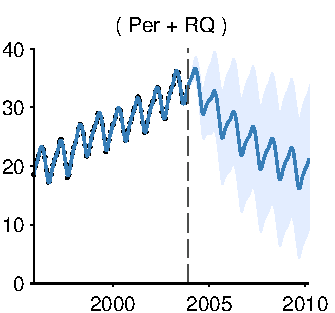
\includegraphics[width=\wmg,height=\hmg, clip,trim=0mm 0mm 0mm 7mm]{\grammarfiguresdir/decomposition/11-Feb-v4-03-mauna2003-s_max_level_#1/03-mauna2003-s_all_small}}
\begin{tabular}{ccc}
Level 1: & Level 2: & Level 3: \\
\RQ & $\Per + \RQ$ & $\SE \kerntimes (\Per + \RQ )$ \\[0.5em]
%Level 1: \RQ & Level 2: $\Per + \RQ$ & Level 3: $\SE \kerntimes (\Per + \RQ )$ \\[0.5em]
\maunadecomp{0} & \maunadecomp{1} & \maunadecomp{2} \\[0.5em]
\end{tabular}
\caption[Progression of models as the search depth increases]
{Posterior mean and variance for different depths of kernel search on the Mauna Loa dataset.
The dashed line marks the end of the dataset.
\emph{Left:} First, the function is only modeled as a locally smooth function, and the extrapolation is poor.
\emph{Middle:} A periodic component is added, and the extrapolation improves.
\emph{Right:} At depth 3, the kernel can capture most of the relevant structure, and is able to extrapolate reasonably.
}
\label{fig:mauna_grow}
\end{figure}

\Cref{fig:mauna_search_tree} shows an example search tree followed by our algorithm.
\Cref{fig:mauna_grow} shows how the resulting model changes as the search is followed.
In practice, we also include extra operators which propose commonly-occuring structures, such as changepoints.
A complete list is contained in appendix~\ref{sec:search-operators}.

Our search operators have rough parallels with strategies used by human researchers to construct regression models.
In particular,
\begin{itemize}
\item One can look for structure in the residuals of a model, such as periodicity, and then extend the model to capture that structure.
This corresponds to adding a new kernel to the existing structure.
\item One can start with structure which is assumed to hold globally, such as linearity, but find that it only holds locally.
This corresponds to multiplying a kernel structure by a local kernel such as $\kSE$.
\item One can incorporate input dimensions incrementally, analogous to algorithms like boosting, back-fitting, or forward selection.
This corresponds to adding or multiplying with kernels on dimensions not yet included in the model.
\end{itemize}

%We stop the procedure at a fixed depth (typically 10), and return the best-scoring kernel over all depths.
%The fixed depth was enforcing solely for convencience - because the 




\subsubsection{Hyperparameter initialization}

Unfortunately, optimizing the marginal likelihood over parameters is not a convex optimization problem, and the space can have many local optima.
For example, in data having periodic structure, integer multiples of the true period (harmonics) are often local optima. 
We take advantage of our search procedure to provide reasonable initializations: all parameters which were part of the previous kernel are initialized to their previous values. Newly introduced paramters are initialized randomly.
In the newly proposed kernel, all parameters are then optimized using conjugate gradients.
This procedure is not guaranteed to find the global optimum, but it implements the commonly used heuristic of iteratively modeling residuals.






\section{A model comparison procedure}

Choosing a kernel requires a method for comparing models.
We choose marginal likelihood as our criterion, since it balances the fit and complexity of a model \citep{rasmussen2001occam}.
Conditioned on kernel parameters, the marginal likelihood of a \gp{} can be computed analytically by \cref{eq:gp_marg_lik}.
%Given a parametric form of a kernel, we can also choose its parameters using marginal likelihood.
%However, choosing kernel parameters by maximum likelihood (as opposed to integrating them out) raises the possibility of overfitting.
In addition, if one compares \gp{} models by the maximum likelihood value obtained after optimizing their kernel parameters, then all else being equal, the model having more free parameters will be chosen.
This introduces a bias in favor of more complex models.

We could avoid overfitting by integrating the marginal likelihood over all free parameters, but this integral is difficult to do in general.
Instead, we loosely approximate this integral using the Bayesian information criterion (\BIC{}) \citep{schwarz1978estimating}:
%
\begin{equation}
\textrm{BIC}(M) = \log p(D \given M) - \frac{1}{2} |M| \log N
\end{equation}
%
where $p(D|M)$ is the marginal likelihood of the data evaluated at the optimized kernel parameters, $|M|$ is the number of kernel parameters, and $N$ is the number of data points.
\BIC{} simply penalizes the marginal likelihood in proportion to how many parameters the model has.
%BIC trades off model fit against model complexity and implements what is known as ``Bayesian Occam's Razor'' \citep{rasmussen2001occam,mackay2003information}.
Because BIC is a function of the number of parameters in a model, we did not count kernel parameters known to not affect the model.
For example, when two kernels are multiplied, one of their output variance parameters becomes redundant, and can be ignored.

Other more sophisticated approximations are possible, such as Laplace's approximation.
We chose to try \BIC{} first because of its simplicity, and it performed reasonably well in our experiments.




\section{A model description procedure}

As discussed in \cref{ch:kernels}, a \gp{} whose kernel is a sum of kernels can be viewed as a sum of functions drawn from different \gp{}s.
We can always express any kernel structure as a sum of products of kernels by distributing all products of sums.
For example,
%
\begin{align}
\SE \kerntimes (\RQ \kernplus \Lin) = \SE \kerntimes  \RQ \kernplus \SE \kerntimes \Lin
\end{align}
%
When all kernels in a product apply to the same dimension, we can use the formulas in \cref{sec:posterior-variance} to visualize the marginal posterior distribution of that component.
This decomposition into additive components provides a method of visualizing \gp{} models which disentangles the different types of structure in the model.

The following section shows examples of such decomposition plots.
In \cref{ch:description}, we will extend this model visualization method to include automatically generated English text explaining types of structure discovered.



\section{Structure discovery in time series}
\label{sec:time_series}

To investigate our method's ability to discover structure, we ran the kernel search on several time-series.
In the following example, the search was run to depth 10, using \kSE{}, \kRQ{}, \kLin{}, \kPer{} and \kWN{} as base kernels.

\begin{figure}[ht!]
\newcommand{\wmgd}{0.5\columnwidth}  % width mauna decomp
\newcommand{\hmgd}{3.51cm}  % height mauna decomp
\newcommand{\mdrd}{\grammarfiguresdir/decomposition/11-Feb-03-mauna2003-s}  % mauna decomp results dir
\newcommand{\mbm}{\hspace{-0.2cm}}  % move back
\newcommand{\maunadgfx}[1]{\mbm \includegraphics[width=\wmgd,height=\hmgd, clip, trim=0mm 0mm 0mm 6mm]{\mdrd/03-mauna2003-s_#1}}
\begin{tabular}{cc}
\multicolumn{2}{c}{
\begin{tabular}{c}
Complete model: 
$\kLin \kerntimes \kSE \kernplus \kSE \kerntimes ( \kPer \kernplus \RQ ) \kernplus \kWN$ \\
\maunadgfx{all}
\end{tabular}
} \\\\
%\multicolumn{2}{c}{Decomposition} \\
Long-term trend: $\Lin \kerntimes \SE$ & Yearly periodic: $\SE \kerntimes \Per$ \\
\maunadgfx{1} & \maunadgfx{2_zoom} \\[1em]
Medium-term deviation: $\SE \kerntimes \RQ$ & Noise: \kWN \\
\maunadgfx{3} & \maunadgfx{resid}
\end{tabular}
\caption[Decomposition of the Mauna Loa model]
{\emph{First row:} The full posterior on the Mauna Loa dataset, after a search of depth 10.
\emph{Subsequent rows:} The automatic decomposition of the time series.
The model is a sum of long-term, yearly periodic, medium-term components, and residual noise, respectively.
The yearly periodic component has been rescaled for clarity.}
\label{fig:mauna_decomp}
\end{figure}

\label{sec:extrapolation}
\subsection{Mauna Loa atmospheric CO$\mathbf{_{2}}$}

First, our method analyzed records of carbon dioxide levels recorded at the Mauna Loa observatory~\citep{co2data}.
Since this dataset was analyzed in detail by \citet[chapter 5]{rasmussen38gaussian}, we can compare the kernel chosen by our method to a kernel constructed by human experts.

\Cref{fig:mauna_grow} shows the posterior mean and variance on this dataset as the search depth increases.
While the data can be smoothly interpolated by a model with only a single base kernel, the extrapolations improve dramatically as the increased search depth allows more structure to be included.

\Cref{fig:mauna_decomp} shows the final model chosen by our method together with its decomposition into additive components.
The final model exhibits plausible extrapolation and interpretable components: a long-term trend, annual periodicity, and medium-term deviations.
These components have similar structure to the kernel hand-constructed by \citet[chapter 5]{rasmussen38gaussian}:
%
\begin{align}
\underwrite{\kSE}{\small long-term trend}
\kernplus
\underwrite{\kSE \kerntimes \kPer}{\small yearly periodic}
\kernplus
\underwrite{\kRQ}{\small medium-term irregularities}
\kernplus 
\underwrite{\kSE \kernplus \kWN}{\small short-term noise}
\end{align}

We also plot the residuals modeled by a white noise ($\kWN$) component, showing that there is little obvious structure left in the data.
More generally, some components capture slowly-changing structure while others capture quickly-varying struture, but often there is no hard distinction between ``signal'' components and ``noise'' components.

\begin{figure}[ht!]
\centering
\newcommand{\wagd}{0.48\columnwidth}  % width airline decomp
\newcommand{\hagd}{4cm}  % height airline decomp
\newcommand{\mb}{\hspace{-0.2cm}}  % move back
%\newcommand{\ard}{../figures/decomposition/11-Feb-01-airline-s}  % airline results dir
%\newcommand{\ard}{\grammarfiguresdir/decomposition/31-Jan-v301-airline-months}  % airline results dir
%
% Level 5 of 
% https://github.com/jamesrobertlloyd/gpss-research/blob/master/results/2014-01-14-GPSS-add/01-airline_result.txt
%SumKernel(SqExp, Product[NoiseKernel LinearKernel], ProductKernel[SqExp, PeriodicKernel, LinearKernel, ProductKernel[SqExpKernel, LinearKernel])])
\newcommand{\ard}{\grammarfiguresdir/decomposition/19-Jan-2014-airline-months}  % airline results dir
\newcommand{\airdgfx}[1]{\mb \includegraphics[width=\wagd,height=\hagd, clip, trim=10mm 0mm 14mm 8mm]{\ard/#1} }
%
\begin{tabular}{cc}
\multicolumn{2}{c}{
\begin{tabular}{c}
Complete Model: $\kSE \kerntimes \Lin \kernplus \kPer \kerntimes \kLin \kerntimes \kSE \kernplus \kLin \kerntimes \kSE \kernplus \kWN \kerntimes \kLin$ \\
\airdgfx{01-airline_all} \\
%{\mb 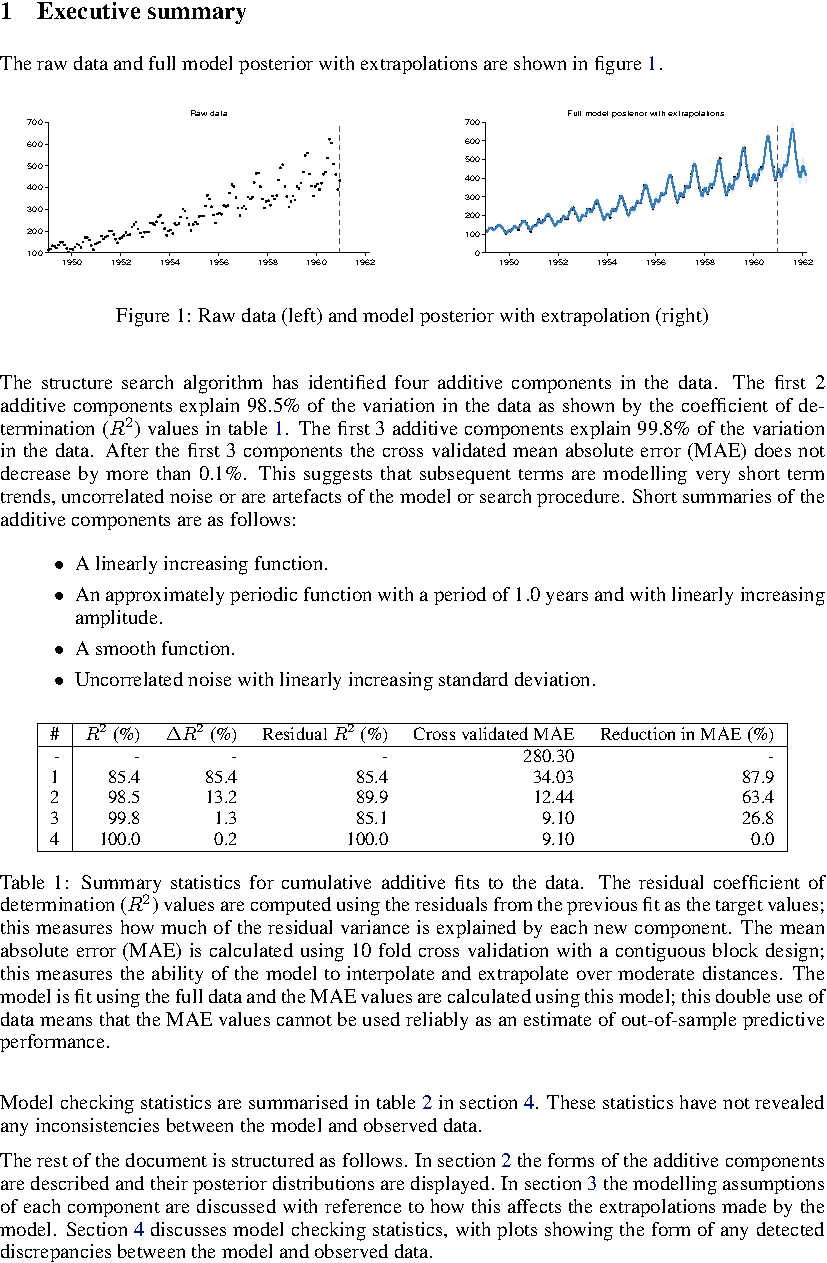
\includegraphics[width=\wagd,height=\hagd, clip, trim=4.5mm 60mm 77mm 37.3mm]{\grammarfiguresdir/airlinepages/pg_0002-crop} }
\end{tabular}
} \\
Long-term trend: $\kSE \kerntimes \kLin$ & Yearly periodic: $\kPer \kerntimes \Lin \kerntimes \kSE$ \\
%{\mb 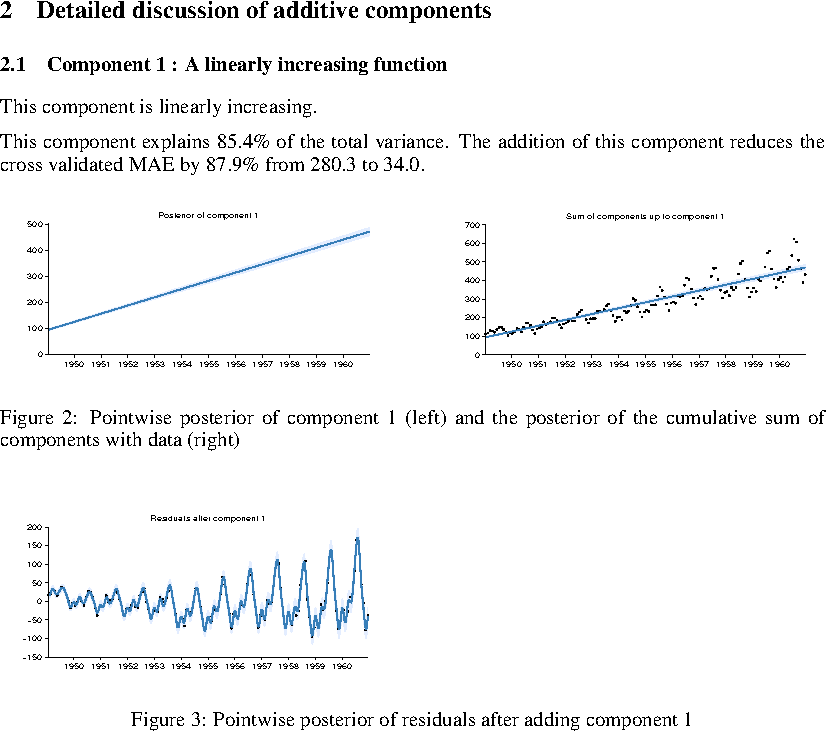
\includegraphics[width=\wagd,height=\hagd, clip, trim=4.5mm 60mm 77mm 37.3mm]{\grammarfiguresdir/airlinepages/pg_0003-crop} } &
\airdgfx{01-airline_1_extrap} & 
\airdgfx{01-airline_2_extrap} \\
%{\mb 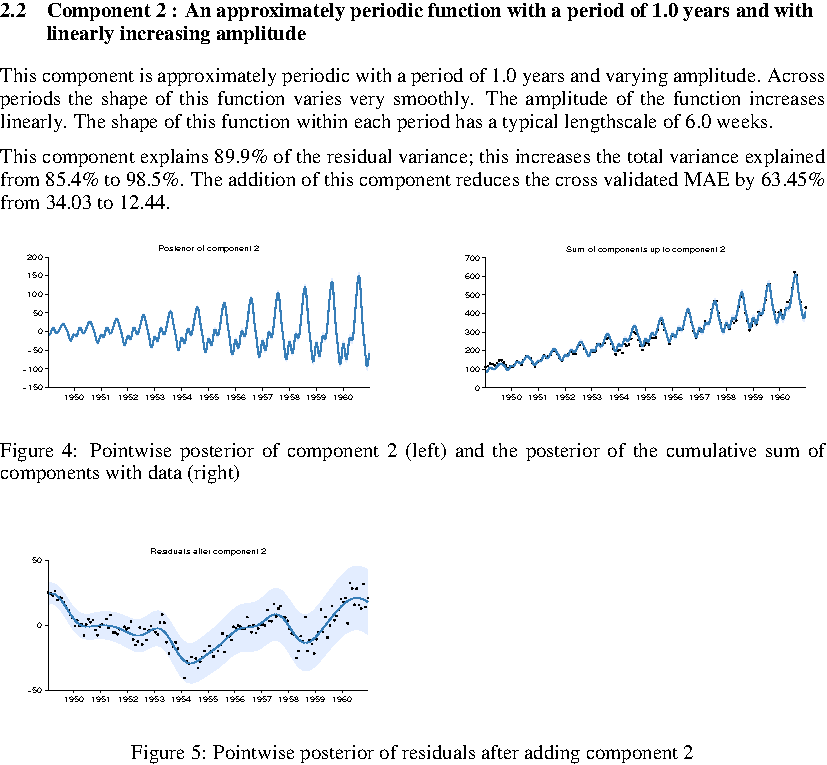
\includegraphics[width=\wagd,height=\hagd, clip, trim=4.5mm 60mm 77mm 43mm]{\grammarfiguresdir/airlinepages/pg_0004-crop} } \\
Medium-term deviation: $\kSE$ & Growing noise: $\kWN \kerntimes \Lin$ \\
\airdgfx{01-airline_3_extrap} & 
%{\mb 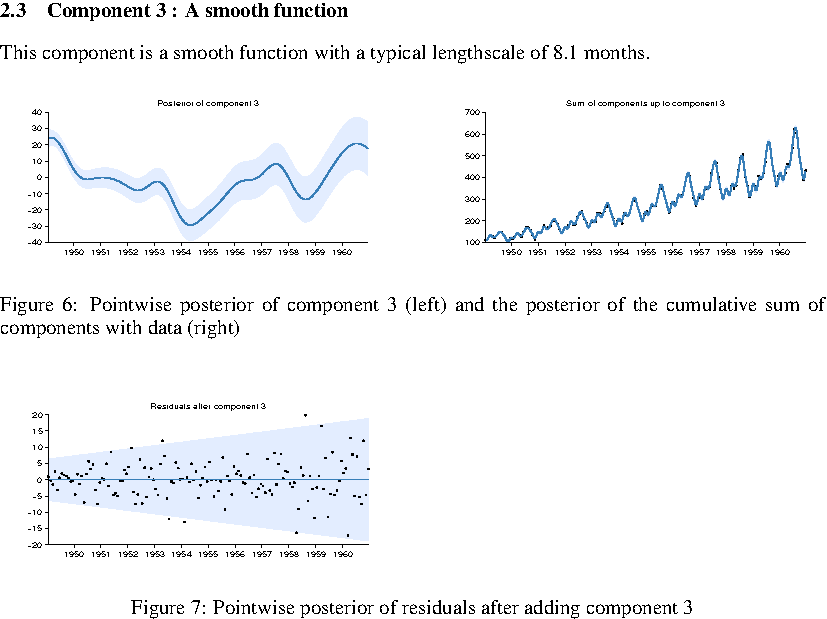
\includegraphics[width=\wagd,height=\hagd, clip, trim=5mm 60mm 77mm 18.5mm]{\grammarfiguresdir/airlinepages/pg_0005-crop} } &
%\airdgfx{01-airline_4_extrap} 
{\mb 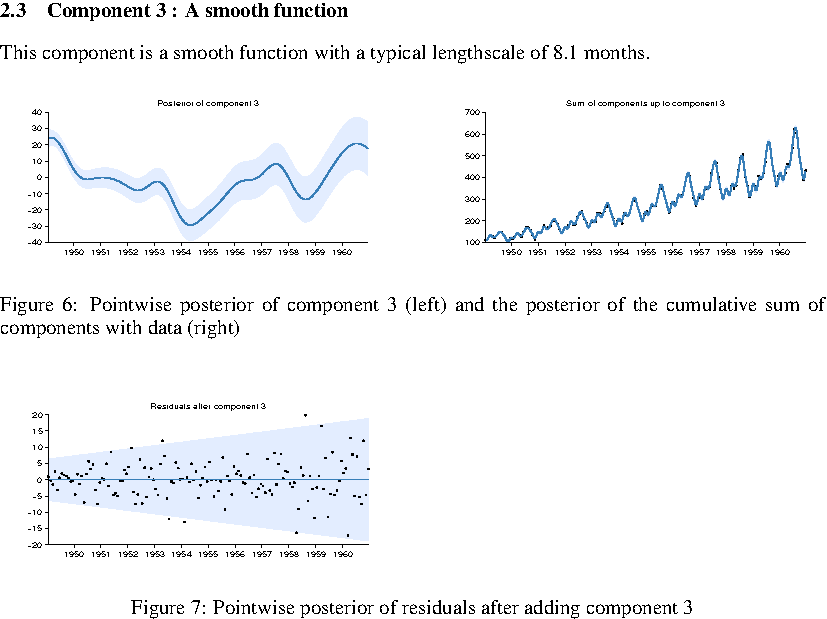
\includegraphics[width=\wagd,height=\hagd, clip, trim=5mm 8.5mm 7.8cm 69.5mm]{\grammarfiguresdir/airlinepages/pg_0005-crop} }
\end{tabular}
\caption[Decomposition of airline dataset model]
{\emph{First row:} The airline dataset and posterior after a search of depth 10.
\emph{Subsequent rows:} Additive decomposition of posterior into long-term smooth trend, yearly variation, and short-term deviations.
Due to the linear kernel, the marginal variance grows over time, making this a heteroskedastic model. 
}
\label{fig:airline_decomp}
\end{figure}

\subsection{Airline passenger counts}

\Cref{fig:airline_decomp} shows the decomposition produced by applying our method to monthly totals of international airline passengers~\citep{box2013time}.
We observe similar components to those in the Mauna Loa dataset: a long term trend, annual periodicity, and medium-term deviations.
In addition, the composite kernel captures the near-linearity of the long-term trend, and the linearly growing amplitude of the annual oscillations.

% Created by the command:
% postprocessing.make_all_1d_figures(folder='../results/31-Jan-1d/', prefix='31-Jan-v3', rescale=False)


The model search can be run without modification on multi-dimensional datasets (as in \cref{sec:synthetic,sec:additive-experiments}), but the resulting structures are more difficult to visualize.


\section{Related work}
\label{sec:gpss-related-work}

\def\rwsheader{\subsubsection}

\rwsheader{Building kernel functions by hand}
\citet[chapter 5]{rasmussen38gaussian} devoted 4 pages to manually constructing a composite kernel to model the Mauna Loa dataset.
%In the supplementary material, we include a report automatically generated by \procedurename{} for this dataset; our procedure chose a model similar to the one they constructed by hand.
Other examples of papers whose main contribution is to manually construct and fit a composite \gp{} kernel are \citet{textperiodic13}, \citet{lloydgefcom2012}, and \citet{EdgarTelescope}.
These papers show that experts are capable of constructing kernels, in one or two dimensions, of similar complexity to the ones shown in this chapter.
However, a more systematic search can consider possibilities that might otherwise be missed.
For example, the kernel structure $\kSE \kerntimes \kPer \kerntimes \kLin$, while appropriate for the airline dataset, had never been considered by the authors before it was chosen by the automatic search.



\rwsheader{Nonparametric regression in high dimensions}
Nonparametric regression methods such as splines, locally-weighted regression, and \gp{} regression are capable of learning arbitrary smooth functions from data.
Unfortunately, they suffer from the curse of dimensionality: it is sometimes difficult for these models to generalize well in more than a few dimensions.

Applying nonparametric methods in high-dimensional spaces can require imposing additional structure on the model.
One such structure is additivity.
Generalized additive models~\citep{hastie1990generalized} assume the regression function is a transformed sum of functions defined on the individual dimensions: $\expect[f(\vx)] = g\inv(\sum_{d=1}^D f_d(x_d))$.
These models have a restricted form, but one which is interpretable and often generalizes well.
Models in our grammar can capture similar structure through sums of base kernels along different dimensions, although we have not yet tried incorporating a warping function $g(\cdot)$.

It is possible to extend additive models by adding more flexible interaction terms between dimensions. 
\Cref{ch:additive} considers \gp{} models whose kernel implicitly sums over all possible interactions of input variables.
\citet{plate1999accuracy} constructs a special case of this model class, summing an \kSE{} kernel along each dimension (for interpretability) plus a single \seard{} kernel over all dimensions (for flexibility).
Both types of model can be expressed in our grammar.

A closely related procedure is smoothing-splines \ANOVA{} \citep{wahba1990spline, gu2002smoothing}.
This model is a weighted sum of splines along each input dimension, all pairs of dimensions, and possibly higher-dimensional combinations.
Because the number of terms to consider grows exponentially with the number of dimensions included in each term, in practice, only one- and two-dimensional terms are usually considered.

Semi-parametric regression \citep[e.g.][]{ruppert2003semiparametric} attempts to combine interpretability with flexibility by building a composite model out of an interpretable, parametric part (such as linear regression) and a ``catch-all'' nonparametric part (such as a \gp{} having an \kSE{} kernel).
This model class can be represented through kernels such as ${\kSE \kernplus \kLin}$.


\rwsheader{Kernel learning}
There is a large body of work attempting to construct rich kernels through a weighted sum of base kernels, called multiple kernel learning (\MKL{}) \citep[e.g.][]{gonen2011multiple, bach2004multiple}.
These approaches usually have a convex objective function.
However the component kernels, as well as their parameters, must be specified in advance.
We compare to a Bayesian variant of \MKL{} in \cref{sec:numerical}, expressed as a restriction of our language of kernels.

\citet{salakhutdinov2008using} use a deep neural network with unsupervised pre-training to learn an embedding $g(\vx)$ onto which a \gp{} with an $\kSE$ kernel is placed: ${\Cov{[f(\vx), f(\vx')]} = k(g(\vx), g(\vx'))}$.
This is a flexible approach to kernel learning, but relies mainly on finding structure in the input density $p(\vx)$.
Instead, we focus on domains where most of the interesting structure is in $f(\vx)$.

Sparse spectrum \gp{}s \citep{lazaro2010sparse} approximate the spectral density of a stationary kernel function using sums of Dirac delta functions, which corresponds to kernels of the form $\sum \cos$.
Similarly, \citet{WilAda13} introduced spectral mixture kernels, which approximate the spectral density using a mixture of Gaussians, corresponding to kernels of the form $\sum \kSE \kerntimes \cos$.
Both groups demonstrated, using Bochner's theorem \citep{bochner1959lectures}, that these kernels can approximate any stationary covariance function.
Our language of kernels includes both of these kernel classes (see \cref{table:motifs}).


\rwsheader{Changepoints}

There is a wide body of work on changepoint modeling.
\citet{adams2007bayesian} developed a Bayesian online changepoint detection method which segments time-series into independent parts.
This approach was extended by \citet{saatcci2010gaussian} to Gaussian process models.
\citet{garnett2010sequential} developed a family of kernels which modeled changepoints occurring abruptly at a single point.
The changepoint kernel (\kCP) presented in this work is a straightforward extension to smooth changepoints.


\rwsheader{Equation learning}
\cite{todorovski1997declarative}, \cite{washio1999discovering} and \cite{Schmidt2009b} learned parametric forms of functions, specifying time series or relations between quantities.
In contrast, \procedurename{} learns a parametric form for the covariance function, allowing it to model functions which do not have a simple parametric form but still have high-level structure.
An examination of the structure discovered by the automatic equation-learning software Eureqa \citep{Eureqa} on the airline and Mauna Loa datasets can be found in \citet{LloDuvGroetal14}.
%\Cref{sec:eqn-learning-comp}.



\rwsheader{Structure discovery through grammars}

\citet{kemp2008discovery} learned the structural form of graphs that modeled human similarity judgements.
Their grammar on graph structures includes planes, trees, and cylinders.
Some of their discrete graph structures have continuous analogues in our language of models.
For example, $\SE_1 \kerntimes \SE_2$ and $\SE_1 \kerntimes \Per_2$ can be seen as mapping the data onto a Euclidian surface and a cylinder, respectively.
\Cref{sec:topological-manifolds} examined these structures in more detail.

\citet{diosan2007evolving} and \citet{bing2010gp} learned composite kernels for support vector machines and relevance vector machines, respectively, using genetic search algorithms to optimize cross-validation error.
Similarly, \citet{kronberger2013evolution} searched over composite kernels for \gp{}s using genetic programming, optimizing the unpenalized marginal likelihood.
These methods explore similar languages of kernels to the one explored in this chapter.
%However, each of these methods suffer either from a model selection criterion which is not differentiable with respect to kernel parameters (cross-validation of classification accuracy), or from one which does not penalize complexity of the resulting kernel expressions.
It is not clear whether the complex genetic searches used by these methods offer advantages over the straightforward but na\"{i}ve greedy search used in this chapter.
%However, \citet{kronberger2013evolution} observed overfitting
%Our work goes beyond ths prior work by demonstrating the structure implied by composite kernels, employing a Bayesian search criterion, and allowing for the automatic discovery of interpretable structure from data.
Our search criterion has the advantages of being both differentiable with respect to kernel parameters, and of trading off model fit and complexity automatically.
These related works also did not explore the automatic model decomposition, summarization and description made possible by the use of \gp{} models.
% and goes beyond this prior work by demonstrating the interpretability of the structure implied by composite kernels, and how such structure allows for extrapolation.


\citet{grosse2012exploiting} performed a greedy search over a compositional model class for unsupervised learning, using a grammar of matrix decomposition models, and a greedy search procedure based on held-out predictive likelihood.
This model class contains many existing unsupervised models as special cases, and was able to discover diverse forms of structure, such as co-clustering or sparse latent feature models, automatically from data.
Our framework takes a similar approach, but in a supervised setting.

Similarly, \citet{christian-thesis} showed to automatically perform inference in arbitrary compositions of discrete sequence models.
More generally, \citet{dechter2013bootstrap} and \citet{liang2010learning} constructed grammars over programs, and automatically searched the resulting spaces.




\section{Experiments}
\label{sec:numerical}

\subsection{Interpretability versus accuracy}

BIC trades off model fit and complexity by penalizing the number of parameters in a kernel expression.
This can result in \procedurename{} favoring kernel expressions with nested products of sums, producing descriptions involving many additive components after expanding out all terms.
While these models typically have good predictive performance, their large number of components can make them less interpretable.
We experimented with not allowing parentheses during the search, discouraging nested expressions.
This was done by distributing all products immediately after each search operator was applied.
We call this procedure \procedurename{}-interpretability, in contrast to the unrestricted version of the search, \procedurename{}-accuracy.


\subsection{Predictive accuracy on time series}
\label{sec:Predictive accuracy on time series}

%\subsubsection{Datasets}

We evaluated the performance of the algorithms listed below on 13 real time-series from various domains from the time series data library \citep{TSDL}.
The pre-processed datasets used in our experiments are available at \\\url{http://github.com/jamesrobertlloyd/gpss-research/tree/master/data/tsdlr}
% plots of the data can be found at the beginning of the reports in the supplementary material.



\subsubsection{Algorithms}

We compare \procedurename{} to equation learning using Eureqa \citep{Eureqa}, as well as six other regression algorithms:
linear regression,
\gp{} regression with a single $\kSE$ kernel (squared exponential),
a Bayesian variant of multiple kernel learning (\MKL{}) \citep[e.g.][]{gonen2011multiple, bach2004multiple},
changepoint modeling \citep[e.g.][]{garnett2010sequential, saatcci2010gaussian, FoxDunson:NIPS2012},
spectral mixture kernels \citep{WilAda13} (spectral kernels),
and trend-cyclical-irregular models \citep[e.g.][]{lind2006basic}.

We set Eureqa's search objective to the default mean-absolute-error.
All algorithms besides Eureqa can be expressed as restrictions of our modeling language (see \cref{table:motifs}), so we performed inference using the same search and objective function, with appropriate restrictions to the language.
%For \MKL{}, trend-cyclical-irregular, and spectral kernels, the greedy search procedure of \procedurename{} corresponds to a forward-selection algorithm.
%For squared-exponential and linear regression, the procedure corresponds to standard marginal likelihood optimization.
%More advanced inference methods are sometimes used for changepoint modeling, but we use the same inference method for all algorithms for comparability.

We restricted our experiments to regression algorithms for comparability; we did not include models which regress on previous values of times series, such as auto-regressive or moving-average models \citep[e.g.][]{box2013time}.
Constructing a language of autoregressive time-series models would be an interesting area for future research.



\subsubsection{Extrapolation experiments}

To test extrapolation, we trained all algorithms on the first 90\% of the data, predicted the remaining 10\% and then computed the root mean squared error (\RMSE{}).
The \RMSE{}s were then standardised by dividing by the smallest \RMSE{} for each data set, so the best performance on each data set has a value of 1.

\begin{figure}[h!]
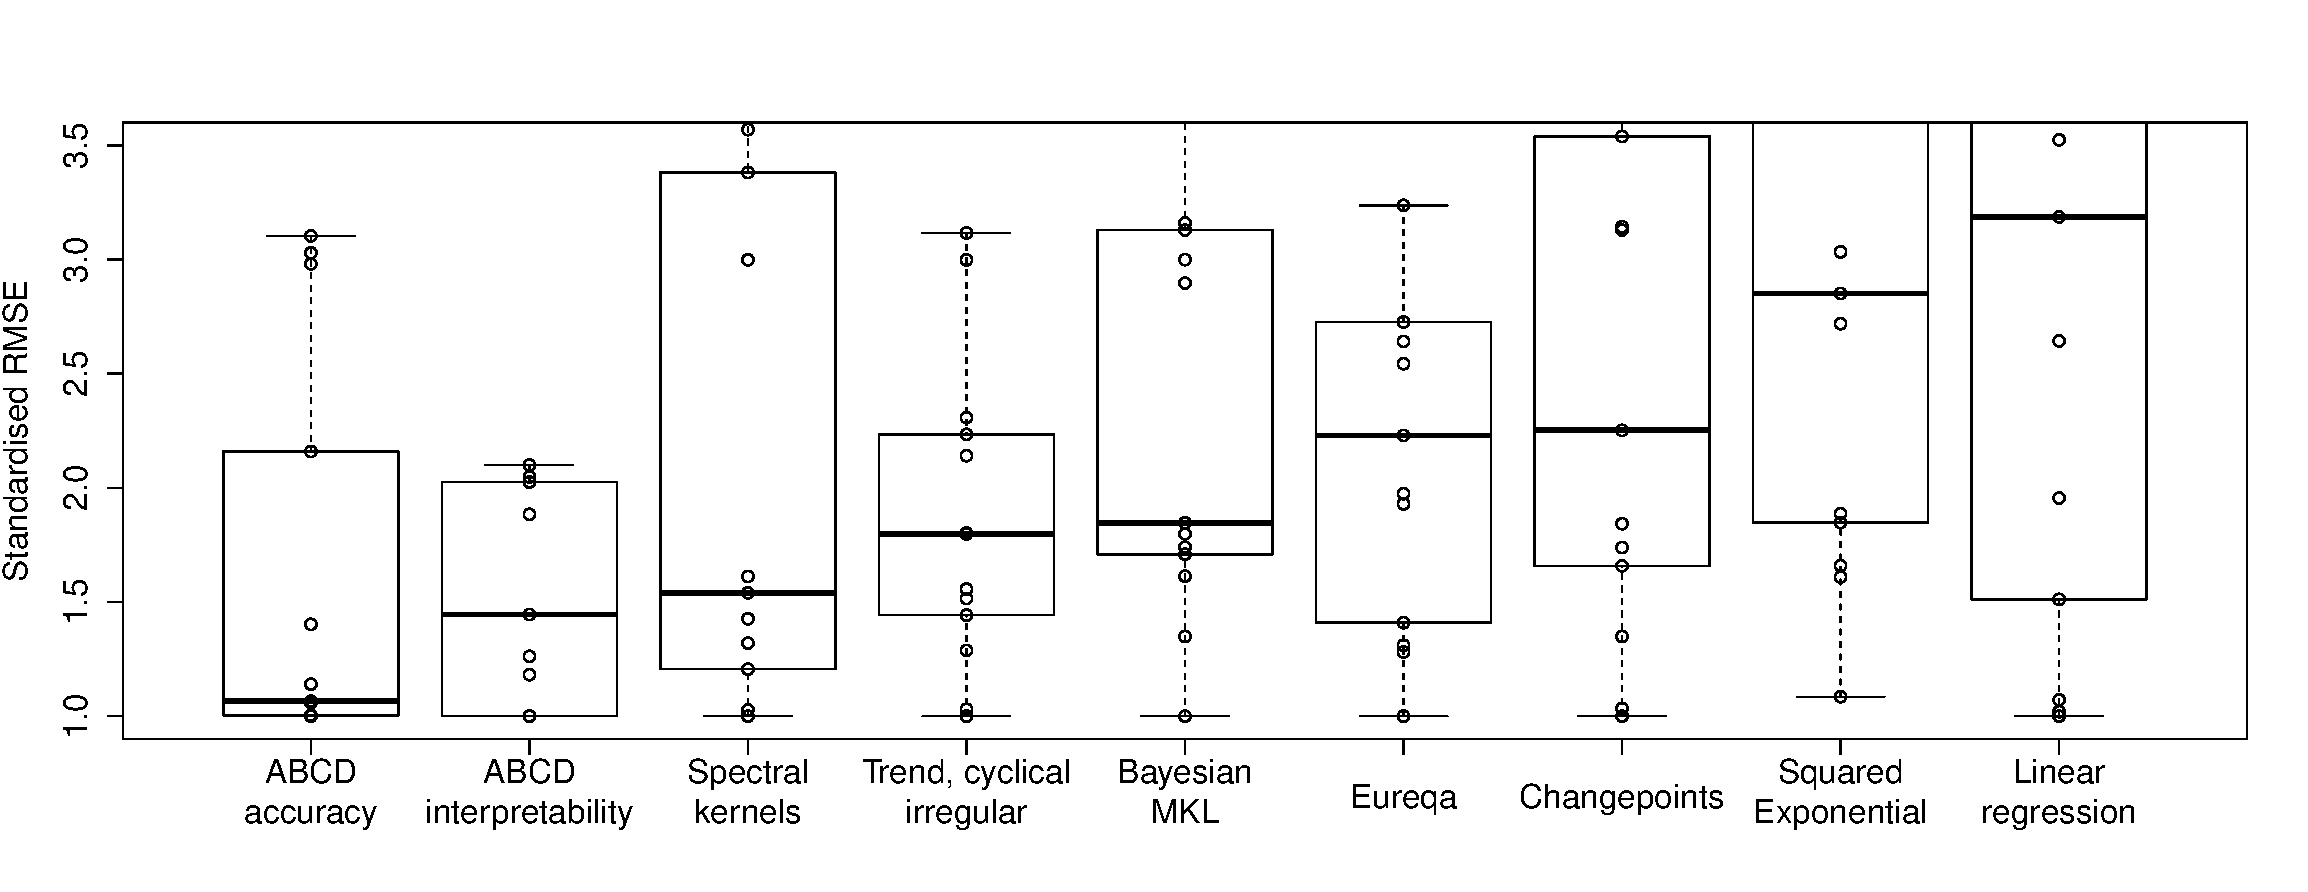
\includegraphics[width=1.02\textwidth]{\grammarfiguresdir/comparison/box_extrap_wide}
\caption[Extrapolation error of all methods on 13 time-series datasets]
{Box plot (showing median and quartiles) of standardised extrapolation \RMSE{} (best performance = 1) on 13 time-series.
Methods are ordered by median.
}
\label{fig:box_extrap_dist}
\end{figure}


\Cref{fig:box_extrap_dist} shows the standardised \RMSE{}s across algorithms.
\procedurename{}-accuracy usually outperformed \procedurename{}-interpretability.
Both algorithms had lower quartiles than all other methods.

Overall, the model construction methods having richer languages of models performed better: \procedurename{} outperformed trend-cyclical-irregular, which outperformed Bayesian \MKL{}, which outperformed squared-exponential.
Despite searching over a rich model class, Eureqa performed relatively poorly.
This may be because few datasets are parsimoniously explained by a parametric equation, or because of the limited regularization ability of this procedure.

Not shown on the plot are large outliers for spectral kernels, Eureqa, squared exponential and linear regression with normalized \RMSE{}s of 11, 493, 22 and 29 respectively.
%All of these outliers occurred on a data set with a large discontinuity (see the call centre data in the supplementary material).

%\subsubsection{Interpolation}
%To test the ability of the methods to interpolate, we randomly divided each data set into equal amounts of training data and testing data.
%The results are similar to those for extrapolation, and are included in \cref{sec:interpolation-appendix}.

%\fTBD{Josh: Can you write about the Blessing of abstraction, and doing lots with a small amount of data?  This might become apparent from plotting the extraplolations.}
%\fTBD{RBG: We could make this point as part of the learning curves for extrapolation by marking the points at which each additional aspect of the structure is found.}





\subsection{Multi-dimensional prediction}

\procedurename{} can be applied to multidimensional regression problems without modification.
An experimental comparison with other methods can be found in \cref{sec:additive-experiments}, where it has the best performance on every dataset.%outperforms a wide variety of multidimensional regression methods.



\subsection{Structure recovery on synthetic data}
\label{sec:synthetic}

The structure found in the examples above may seem reasonable, but we may wonder to what extent \procedurename{} is consistent -- that is, does it recover all the structure in any given dataset?
It is difficult to tell from predictive accuracy alone if the search procedure is finding the correct structure, especially in multiple dimensions.
To address this question, we tested our method's ability to recover known structure on a set of synthetic datasets.

For several composite kernel expressions, we constructed synthetic data by first sampling 300 locations uniformly at random, then sampling function values at those locations from a \gp{} prior.
We then added \iid Gaussian noise to the functions at various signal-to-noise ratios (\SNR{}).


\begin{table}[ht!]
\caption[Kernels chosen on synthetic data]
{
Kernels chosen by \procedurename{} on synthetic data generated using known kernel structures.
$D$ denotes the dimension of the function being modeled.
\SNR{} indicates the signal-to-noise ratio.
Dashes (--) indicate no structure was found.
Each kernel implicitly has a \kWN{} kernel added to it.
}
\label{tbl:synthetic}
\addtolength{\tabcolsep}{1pt}
\setlength\extrarowheight{2pt}
\begin{center}
{\small
\begin{tabular}{c c | c c c}
True kernel & $D$ & \SNR{} = 10 & \SNR{} = 1 & \hspace{-1cm} \SNR{} = 0.1 \\
\hline
$\SE \kernplus \RQ$        & 1 & $\SE$ & $\SE \kerntimes \Per$ & $\SE$ \\
$\Lin \kerntimes \Per$ & 1 & $\Lin \kerntimes \Per$ & $\Lin \kerntimes \Per$ & $\SE$ \\
$\SE_1 \kernplus \RQ_2$    & 2 & $\SE_1 \kernplus \SE_2$ & $\Lin_1 \kernplus \SE_2$ & $\Lin_1$ \\
$\SE_1 \kernplus \SE_2 \kerntimes \Per_1 \kernplus \SE_3$ & 3 & $\SE_1 \kernplus \SE_2 \kerntimes \Per_1 \kernplus \SE_3$ & $\SE_2 \kerntimes \Per_1 \kernplus \SE_3$ & -- \\
$\SE_1 \kerntimes \SE_2$ & 4 & $\SE_1 \kerntimes \SE_2$ & $\Lin_1 \kerntimes \SE_2$ & $\Lin_2$ \\
$\SE_1 \kerntimes \SE_2 \kernplus \SE_2 \kerntimes \SE_3$ & 4 & $\SE_1 \kerntimes \SE_2 \kernplus \SE_2 \kerntimes \SE_3$ & $\SE_1 \kernplus \SE_2 \kerntimes \SE_3$ & $\SE_1$ \\
\multirow{2}{*}{ $(\SE_1 \kernplus \SE_2) \kerntimes (\SE_3 \kernplus \SE_4)$ } & \multirow{2}{*}{4} & $(\SE_1 \kernplus \SE_2) \, \kerntimes$ \dots & $(\SE_1 \kernplus \SE_2) \, \kerntimes$ \dots & \multirow{2}{*}{--} \\
 & & $(\SE_3\kerntimes\Lin_3\kerntimes\Lin_1 \kernplus \SE_4)$ & $\SE_3 \kerntimes \SE_4$ &
\end{tabular}
}
\end{center}
\end{table}


\Cref{tbl:synthetic} shows the results.
For the highest signal-to-noise ratio, \procedurename{} finds all relevant structure except in one case.
The reported additional linear structure in the last row can be explained the fact that functions sampled from \kSE{} kernels with long length-scales occasionally have near-linear trends.
As the noise increases, our method generally backs off to simpler structures rather than over-fitting.

\subsubsection{Source code}
All \gp{} parameter optimization was performed by automated calls to the \GPML{} toolbox~\citep{GPML}.
%, available at \url{http://www.gaussianprocess.org/gpml/code}.
Source code to perform all experiments is available at \url{http://www.github.com/jamesrobertlloyd/gp-structure-search}.




\section{Conclusion}

This chapter presented a system which constructs a model from an open-ended language, and automatically generates plots decomposing the different types of structure present in the model.

This was done by introducing a space of kernels defined by sums and products of a small number of base kernels.  
The set of models in this space includes many standard regression models.
We proposed a search procedure for this space of kernels, and argued that this search process parallels the process of model-building by statisticians.

We found that the learned structures enable relatively accurate extrapolation in time-series datasets. %, and are competitive with widely used kernel classes on a variety of prediction tasks.
The learned kernels can yield decompositions of a signal into diverse and interpretable components, enabling model-checking by humans.
We hope that this procedure has the potential to make powerful statistical model-building techniques accessible to non-experts.

Some discussion of the limitations of this approach to model-building can be found in \cref{sec:limitations-of-abcd}, and discussion of this approach relative to other model-building approaches can be found in \cref{top-down-vs-bottom-up}.
The next chapter will show how the model components found by \procedurename{} can be automatically described using English-language text.




\iffalse
\section{Future Work}

\subsubsection{Structure search in classification}
While we focus on Gaussian process regression, the kernel search method could be applied to other supervised learning problems such as classification or ordinal regression.
%, or to other kinds of kernel architectures such as kernel \SVM{}s.
However, it might be more difficult to discover structure from class labels alone, since they usually contain less information about the underlying process than regression targets.
%However, whether or not such modularity and interpretability is present in other model classes is an open question.

\subsubsection{Improving the search}
The search procedure used in this chapter leaves much room for improvement.
Presumably, some sort of model-based search would be worthwhile, since evaluating each kernel expression is relatively expensive.
This raises the question of how to build an open-ended model of the relative marginal likelihood of \gp{} models.
In order to use a \gp{} for this task, one would need to create a kernel over kernels, as in \citet{ong2002hyperkernels}.

One interesting possibility is that the model of model performance could generate its own data offline.
The system could generate synthetic regression datasets, then score many kernel structures on those datasets in order to improve its model of kernel performance.

%\subsubsection{Building languages of other model classes}
%The compositionality of diverse types of kernels is what allowed a rich language of \gp{} models.
%Can we build similar languages of other model classes?

%As noted in \cref{sec:gpss-related-work}, languages have already been constructed on several powerful model classes: matrix decompositions, sequence models, graphical models, and functional programs.
%Building languages of models that support efficient search as well as interpretable decompositions could be a fruitful direction.
%\citet{roger-grosse-thesis} demonstrated a very rich class of unsupervised models by composing matrix decompositions.
%\citet{kemp2008discovery} and \citet{ellislearning} built grammars on graphical models.

\subsubsection{Use in model-based optimization}
The automatic model-building procedure described in this chapter could also be used in the inner loop of \gp{}-based Bayesian optimization routines, such as \citet{snoek2012practical}.
Discovering structure such as additivity in a problem could be expected to decrease the number of samples needed.


\subsubsection{Incroporating uncertainty in the structure}
\fi


\outbpdocument{
\bibliographystyle{plainnat}
\bibliography{references.bib}
}
